\documentclass[12pt]{article}

\usepackage{sbc-template}
\usepackage{graphicx,url}
\usepackage[utf8]{inputenc}
\usepackage[english,brazilian]{babel}
\usepackage{booktabs}
%\usepackage[latin1]{inputenc}

\sloppy

\title{O Problema do Caminho Mais Curto:\\ Uma Abordagem Empírica
sobre Algoritmos de Roteamento Intra-Domínio}

\author{Álvaro B. Filho\inst{1}, Letícia Q. Wanderley\inst{1}, Luiz
R. S. Pontes\inst{1}, Pedro L. Azevedo\inst{1} }

\address{Instituto Metrópole Digital -- Universidade Federal do Rio
  Grande \\ do Norte
  (UFRN)\\
  \email{\{alvaro.filho.111,leticia.queiroz.109,} \\
  \email{renan.pontes.704,pedro.azevedo.706\}@ufrn.edu.br}
}

\begin{document}

\maketitle

\section{Introdução}

O tema deste trabalho consiste na análise empírica de algoritmos de
roteamento e busca de caminhos mínimos (\textit{shortest path}) em
grafos. Dentro desse contexto, o problema central a ser solucionado
é a determinação da rota de menor custo entre um vértice de origem
e todos os demais vértices presentes em uma rede, uma tarefa
computacional essencial para a comunicação e a atualização de
tabelas de roteamento intra-domínio. Os algoritmos selecionados para
essa análise foram o Algoritmo de Bellman-Ford e o Algoritmo de Dijkstra,
duas abordagens clássicas e com naturezas matemáticas distintas.

O objetivo central deste experimento é investigar empiricamente o
comportamento prático desses algoritmos e relacioná-lo rigorosamente
à sua respectiva análise assintótica. Para alcançar essa meta, o tamanho
da entrada dos grafos será aumentado de forma sistemática com o intuito
de medir o tempo de execução de cada estrutura, comparando o crescimento
temporal observado na prática com a complexidade teórica esperada. Portanto,
espera-se identificar o ponto exato em que a diferença de desempenho entre os
algoritmos se torna significativa, evidenciando a eficiência e as limitações
de cada abordagem.

\section{Algoritmos e fontes}

Para a resolução do problema de roteamento e busca de caminhos
mínimos, utilizamos como base o artigo ``A Study on Contrast and
Comparison between Bellman-Ford algorithm and Dijkstra's algorithm''
\cite{thippeswamy}. A implementação foi construída a partir da lógica
estrutural e dos pseudocódigos fornecidos pelos
autores no artigo, que detalham os procedimentos fundamentais passo
a passo para a execução de ambos os algoritmos. Dessa forma, traduzimos,
com auxílio da inteligência artifical, as instruções matemáticas da
literatura diretamente para a linguagem C++.

\section{Metodologia}

Para a realização dos experimentos, os algoritmos de Bellman-Ford e 
Dijkstra foram adaptados a partir das instruções contidas no artigo e 
dos pseudocódigos originais para a linguagem C++. Nesse sentido, as práticas de 
alocação manual de memória, presentes na literatura base, foram
substituídas por estruturas seguras como std::vector, prevenindo 
vazamentos e garantindo estabilidade durante as medições de desempenho. 
O parâmetro de entrada $n$ foi definido como o número de vértices do grafo, 
adotando a restrição teórica do estudo original onde o número de arestas é 
igual ao número de vértices ($m = n$). Além disso, a geração artificial dos 
grafos priorizou a ausência de arestas com pesos negativos, fornecendo um 
cenário justo e funcional para ambas as abordagens.

Um aspecto metodológico crítico adotado nesta implementação foi a 
preservação da complexidade assintótica do algoritmo de Dijkstra.
Para assegurar que o comportamento em tempo de execução estivesse alinhado à 
complexidade teórica de $O(\vert{}V\vert{}^2)$ documentada no artigo, 
a busca do vértice de menor custo (Extract-Min) foi mantida através 
de uma busca linear convencional, abstendo-se intencionalmente 
do uso de filas de prioridade otimizadas. Por fim, a arquitetura do 
código isolou rigorosamente as etapas de leitura, alocação de memória 
e geração do grafo, utilizando a biblioteca <chrono> exclusivamente 
ao redor da execução dos algoritmos de busca, garantindo que os 
tempos coletados representem estritamente o processamento das rotas.

Para a medição e comparação dos dois algoritmos, foi implementado um
header em C++ responsável por medir o tempo de execução dos
algoritmos de Dijkstra e  Bellman-Ford. A partir dos dados, é gerado
e registrado um arquivo em formato \textit{Comma-Separated Values
(csv)} para estruturar os resultados. Como método de testes,
utilizou-se tamanho de entrada de $200$ até $5000$, dividido em $10$
intervalos iguais, vista a aplicação dos algoritmos em roteamento
intra-domínio, que raramente ultrapassa alguns milhares de arestas e
vértices. Cada $n$ foi iterado 32 vezes, a fim de calcular a média
aritmética e assim obter o tempo médio de execução, garantindo a
integridade da análise diante da variabilidade dos algoritmos.

\section{Análise teórica} \label{sec:analise_teorica}

Para compreender as diferenças de desempenho que serão observadas na
prática, é fundamental estabelecer primeiro a base teórica de cada abordagem.

No caso do algoritmo de Dijkstra, a operação principal consiste em selecionar
iterativamente o vértice não visitado com a menor distância acumulada e, em
seguida, relaxar os custos de suas arestas adjacentes \cite{thippeswamy}.
Na implementação mais simples, a extração desse nó de menor custo requer uma
varredura linear por todos os vértices restantes \cite{thippeswamy}. Como o
algoritmo precisa visitar cada vértice e avaliar suas respectivas conexões, o
tempo de execução resulta na equação $O(|V|^2 + |E|)$, que pode ser
assintoticamente simplificada para $O(|V|^2)$, onde $|V|$ representa o número
de vértices e $|E|$ o número de arestas \cite{thippeswamy}. Dessa forma, em um
cenário de rede onde o número de nós ($n$) é equivalente ao número
de arestas ($m$), o tempo de processamento estimado cresce proporcionalmente
a $2n^2$, confirmando o comportamento de ordem quadrática \cite{thippeswamy}.

Por outro lado, o algoritmo de Bellman-Ford adota uma estratégia estruturalmente
distinta, abdicando da escolha iterativa. Para assegurar que as distâncias
mínimas sejam propagadas com precisão por toda a rede, o algoritmo
executa um laço
de relaxamento sobre o conjunto completo de arestas exatamente $|V|-1$
vezes \cite{thippeswamy}. Devido a essa varredura exaustiva, o tempo
total é regido
pela multiplicação da quantidade de vértices pela de arestas, estabelecendo uma
complexidade assintótica geral de $O(|V| \times |E|)$ \cite{thippeswamy}. Para o
cenário específico onde o número de arestas ($m$) se iguala ao de nós ($n$), a
complexidade computacional do Bellman-Ford é matematicamente descrita
pela função
$27n^2 + 28n + 3$ \cite{thippeswamy}. Portanto, o termo dominante dessa equação
determina uma ordem assintótica $O(n^2)$, que pode ser simplificada
para a proporção
de $27n^2$ \cite{thippeswamy}.

Embora a análise indique um crescimento assintótico quadrático para
ambos os algoritmos
nessas condições, o coeficiente substancialmente maior no Bellman-Ford fornece a
justificativa teórica para o seu tempo de execução prático ser
consideravelmente superior
ao de Dijkstra \cite{thippeswamy}.

\section{Resultados} \label{sec:resultados}

A presente seção apresenta os resultados empíricos coletados a partir
dos algoritmos para fins de comparação entre seus tempos de execução
com base em um tamanho $n$ de suas entradas, neste caso sendo o
número de vértices do grafo avaliado, resumidos na Tabela
\ref{tab:dados_brutos}, sintetizando os tempos médios calculados para
cada variação de tamanho de entrada dos algoritmos.

\begin{table}[hbtp]
  \centering
  \caption{Tempos médios de execução em milissegundos para grafos de
  tamanho $n$.}
  \label{tab:dados_brutos}
  \begin{tabular}{ccc}
    \toprule
    Tamanho da Entrada ($n$) & Dijkstra (ms) & Bellman-Ford (ms) \\
    \midrule
    200 & 0.8 & 1.5 \\
    680 & 9.0 & 17.0 \\
    1160 & 25.7 & 47.4 \\
    1640 & 21.7 & 40.2 \\
    2120 & 58.2 & 109.6 \\
    2600 & 114.6 & 212.1 \\
    3080 & 143.6 & 269.2 \\
    3560 & 185.3 & 343.2 \\
    4040 & 233.4 & 422.9 \\
    4520 & 266.5 & 471.1 \\
    5000 & 335.1 & 613.6 \\
    \bottomrule
  \end{tabular}
\end{table}

Para melhor compreensão comparativa, os dados apresentados foram
plotados nas Figuras \ref{fig:grafico_tempos} e
\ref{fig:grafico_normalizado}, demonstrando visualmente,
respectivamente, o distanciamento entre as curvas de tempo médio de
execução conforme o tamanho da entrada aumenta, e a proximidade
dessas mesmas curvas em relação à curva teórica de complexidade após
a normalização.

\begin{figure}[hbtp]
  \centering
  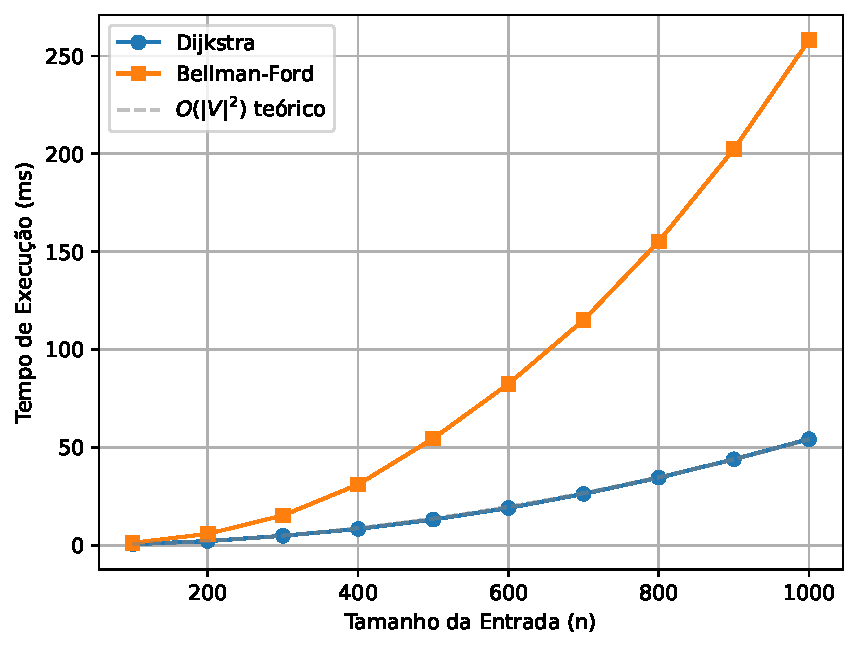
\includegraphics[width=0.8\textwidth]{grafico_tempos.pdf}
  \caption{Comparação do tempo de execução entre Dijkstra e Bellman-Ford.}
  \label{fig:grafico_tempos}
\end{figure}

\begin{figure}[hbtp]
  \centering
  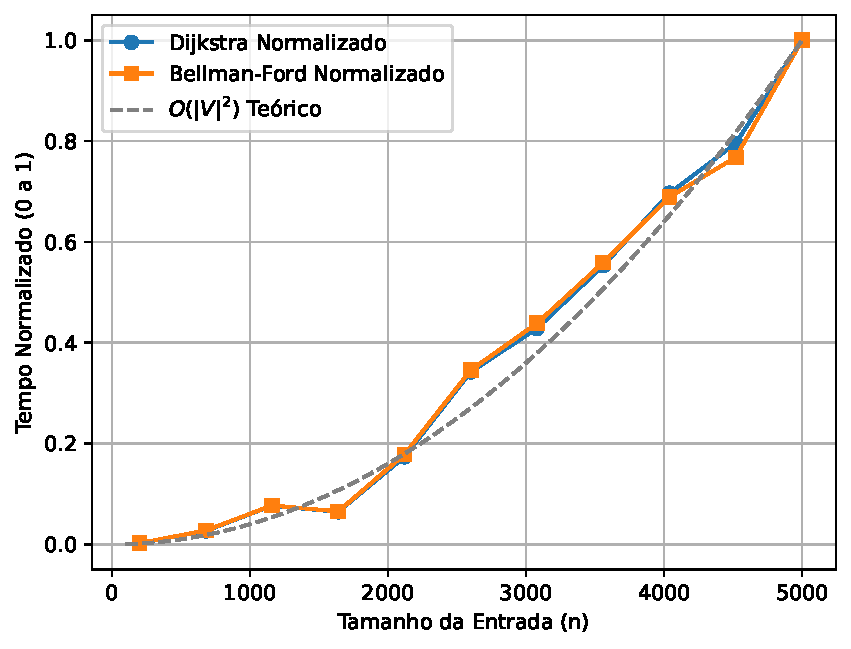
\includegraphics[width=0.8\textwidth]{grafico_normalizado.pdf}
  \caption{Comparação do tempo de execução normalizado entre Dijkstra
  e Bellman-Ford.}
  \label{fig:grafico_normalizado}
\end{figure}

A partir da leitura da Figura \ref{fig:grafico_tempos}, com o tamanho
de entrada ($n$) no eixo x e o tempo de execução (em milissegundos)
no eixo y, observa-se que a diferença absoluta entre as curvas cresce
de forma contínua à medida que o tamanho da entrada aumenta,
refletindo o crescimento polinomial esperado para ambos os
algoritmos. No entanto, ao calcular a razão entre os tempos de
execução do Bellman-Ford e do Dijkstra para cada $n$ da Tabela
\ref{tab:dados_brutos}, observa-se que essa razão permanece
aproximadamente constante ao longo de toda a faixa testada, oscilando
entre $1.77$ e $1.89$ desde as menores até as maiores instâncias
avaliadas. Isso indica que o distanciamento visual observado no
gráfico decorre do crescimento natural de duas curvas de mesma ordem
assintótica com razão fixa entre si, e não de uma mudança de ordem em
algum valor específico de $n$.

Diante disso, ao analisar o eixo x como tamanho de entrada e o eixo
y como o tempo de execução normalizado de 0 a 1 na Figura
\ref{fig:grafico_normalizado}, nota-se que as curvas dos algoritmos
alinham-se de maneira mais próxima à curva teórica de $O(|V|^2)$, sem
apresentar desvios significativos. A normalização, realizada por meio
da divisão da série de dados pelo valor máximo da curva, evidencia
que o perfil de crescimento de ambos os algoritmos reflete a mesma
complexidade polinomial e assintótica, observada pela razão constante
entre as curvas dos algoritmos na Figura \ref{fig:grafico_tempos}.

\section{Discussão}

Sob a ótica dos resultados coletados, observa-se uma eficiência
notavelmente superior do algoritmo de Dijkstra em comparação ao
algoritmo de Bellman-Ford no que diz respeito à busca de caminhos em
roteamento intra-domínio. Os dados empíricos apresentados na Seção
\ref{sec:resultados} corroboram a análise teórica de
\cite{thippeswamy}, fortalecendo a premissa de que, embora ambos
resolvam o problema de busca do caminho mais curto a partir de uma
única origem, o algoritmo de Dijkstra desempenha este papel com menor
custo computacional. Portanto, para quantidades significantes de
arestas, há uma substancial vantagem ao utilizar a busca de menor
caminho por meio de Dijkstra.

Isto ocorre pois o algoritmo de Dijkstra se baseia em uma abordagem
gulosa, ou seja, a cada passo, é realizada uma escolha localmente
ótima, sem reconsiderar escolhas passadas. Para tal, o algoritmo
seleciona o nó de peso mínimo que ainda não foi processado para
realizar o relaxamento das arestas, o que o torna mais eficiente
quando o grafo possui pesos exclusivamente positivos, conforme a
complexidade $O(|V|^2)$ estabelecida na Seção \ref{sec:analise_teorica}.

Em contrapartida, o algoritmo de Bellman-Ford não adota uma
estratégia gulosa: em vez disso, executa a mesma operação de
relaxamento exaustivamente sobre todas as arestas a cada iteração,
repetindo o processo por exatas $|V| - 1$ vezes, como exposto na
Seção \ref{sec:analise_teorica}. Essa varredura exaustiva, embora
mais custosa, é o que confere ao algoritmo a capacidade de processar
corretamente arestas com pesos negativos --- vantagem que o Dijkstra não possui.

Vale destacar que a razão entre os tempos de execução do Bellman-Ford
e do Dijkstra manteve-se estável, entre $1.77$ e $1.89$, mesmo nas
menores instâncias testadas. Isto indica que ambos os algoritmos já
possuem o comportamento assintótico previsto desde $n = 200$, sem um
período inicial em que sejam efetivamente equivalentes. Essa
estabilidade é compatível com a suposição $|E| \approx |V|$ adotada
na Seção \ref{sec:analise_teorica}, sob a qual ambos os algoritmos
assumem ordem quadrática --- o que explica por que nenhuma mudança de
ordem é observada ao longo da faixa avaliada.

Cabe notar, contudo, que a razão prevista pelos polinômios teóricos
levantados naquela seção — $2n^2$ para Dijkstra e $27n^2 + 28n + 3$
para Bellman-Ford, uma razão próxima de $13.5$ — é substancialmente
maior do que a razão observada na prática, de $\approx 1.8$. Essa
discrepância é atribuível a fatores de implementação, como a estrutura de
dados utilizada, efeitos de cache e otimizações do compilador, que não
são capturados pela contagem teórica de operações elementares. Ainda
assim, como a diferença absoluta entre os tempos cresce junto com
$n^2$, o custo de se optar pelo Bellman-Ford em vez do Dijkstra
torna-se cada vez mais significativo em termos práticos à medida que
a rede aumenta, reforçando a preferência pelo Dijkstra em cenários de
roteamento intra-domínio com um número elevado de roteadores e conexões.

\section{Conclusão}

A análise empírica realizada neste trabalho confirma a superioridade
em eficiência do algoritmo de Dijkstra frente ao Bellman-Ford na
busca do caminho mais curto para roteamento intra-domínio. A
abordagem gulosa poupa processamento em comparação à varredura
exaustiva do Bellman-Ford, consolidando o Dijkstra como a escolha
ideal para grafos com pesos estritamente positivos por apresentar
tempos de execução consistentemente menores.

Ainda assim, o algoritmo de Bellman-Ford mantém sua relevância
fundamental em cenários de roteamento que admitem arestas de peso
negativo. Seu elevado custo computacional justifica-se pela
capacidade de encontrar caminhos em redes complexas de forma
confiável. É imperativo ressaltar, contudo, que caso existam ciclos
negativos alcançáveis a partir da origem, nenhum dos algoritmos é
capaz de computar o caminho mais curto, visto que o peso total
decresce infinitamente a cada travessia no ciclo.

Por fim, cabe destacar que os tempos absolutos aferidos nesta análise
são intrínsecos ao \textit{hardware}, sistema operacional e
estruturas de dados utilizados no experimento. Como direcionamento
para trabalhos futuros, sugere-se a execução de testes empíricos em
grafos contendo arestas negativas, a fim de demonstrar na prática a
falha inerente do algoritmo de Dijkstra e a resiliência do
Bellman-Ford diante de tal cenário.

\bibliographystyle{sbc}
\bibliography{sbc-template}

\end{document}
